%%% This file is part of the Open HörTech Master Hearing Aid (openMHA)
%%% Copyright © 2019 2020 2021 HörTech gGmbH
%%% Copyright © 2021 2022 Hörzentrum Oldenburg gGmbH
%%%
%%% openMHA is free software: you can redistribute it and/or modify
%%% it under the terms of the GNU Affero General Public License as published by
%%% the Free Software Foundation, version 3 of the License.
%%%
%%% openMHA is distributed in the hope that it will be useful,
%%% but WITHOUT ANY WARRANTY; without even the implied warranty of
%%% MERCHANTABILITY or FITNESS FOR A PARTICULAR PURPOSE.  See the
%%% GNU Affero General Public License, version 3 for more details.
%%%
%%% You should have received a copy of the GNU Affero General Public License, 
%%% version 3 along with openMHA.  If not, see <http://www.gnu.org/licenses/>.

% Latex header for doxygen 1.8.11
% adapted for openMHA
\documentclass[11pt,a4paper,twoside]{article}

% Packages required by doxygen
\usepackage{fixltx2e}
\usepackage{calc}
\usepackage{../openMHAdoxygen}
\setlength{\headheight}{13.6pt}
\usepackage[export]{adjustbox} % also loads graphicx
\usepackage{graphicx}
\usepackage[utf8]{inputenc}
\usepackage{makeidx}
\usepackage{multicol}
\usepackage{multirow}
\PassOptionsToPackage{warn}{textcomp}
\usepackage{textcomp}
\usepackage[nointegrals]{wasysym}
\usepackage[table]{xcolor}

% Font selection
\usepackage[T1]{fontenc}
\usepackage{helvet}
\usepackage{courier}
\usepackage{amssymb}
\usepackage{sectsty}
\usepackage{textcomp}
\renewcommand{\familydefault}{\sfdefault}
\allsectionsfont{%
  \fontseries{bc}\selectfont%
  \color{darkgray}%
}
\renewcommand{\DoxyLabelFont}{%
  \fontseries{bc}\selectfont%
  \color{darkgray}%
}
\newcommand{\+}{\discretionary{\mbox{\scriptsize$\hookleftarrow$}}{}{}}

% Headers & footers
\usepackage{fancyhdr}
\pagestyle{fancyplain}
\renewcommand{\sectionmark}[1]{%
  \markright{\thesection\ #1}%
}
\fancyhead[LE]{\fancyplain{}{\bfseries\thepage}}
\fancyhead[CE]{\fancyplain{}{}}
\fancyhead[RE]{\fancyplain{}{\bfseries\leftmark}}
\fancyhead[LO]{\fancyplain{}{\bfseries\rightmark}}
\fancyhead[CO]{\fancyplain{}{}}
\fancyhead[RO]{\fancyplain{}{\bfseries\thepage}}
\fancyfoot[LE]{\fancyplain{}{}}
\fancyfoot[CE]{\fancyplain{}{}}
\fancyfoot[RE]{\fancyplain{}{\bfseries\scriptsize \copyright{} 2005-2021 H\"orTech gGmbH, Oldenburg, \bfseries\scriptsize \copyright{} 2021-2022 H\"orzentrum Oldenburg gGmbH }}
\fancyfoot[LO]{\fancyplain{}{\bfseries\scriptsize \copyright{} 2005-2021 H\"orTech gGmbH, Oldenburg, \bfseries\scriptsize \copyright{} 2021-2022 H\"orzentrum Oldenburg gGmbH }}
\fancyfoot[CO]{\fancyplain{}{}}
\fancyfoot[RO]{\fancyplain{}{}}












% Indices & bibliography
\usepackage{natbib}
\usepackage{tocloft}
\setcounter{tocdepth}{2}
\setcounter{secnumdepth}{4}
\addtolength{\cftsubsecnumwidth}{5pt}
\usepackage{fancyvrb}


\RecustomVerbatimCommand{\VerbatimInput}{VerbatimInput}%
{fontsize=\footnotesize,
 %
 frame=lines,  % top and bottom rule only
 framesep=2em, % separation between frame and text
 rulecolor=\color{Gray},
 %
 label=\fbox{\color{Black}data.txt},
 labelposition=topline,
 %
 commandchars=\|\(\), % escape character and argument delimiters for
                      % commands within the verbatim
 commentchar=*        % comment character
}












\makeindex

% Custom commands
\newcommand{\clearemptydoublepage}{%
  \newpage{\pagestyle{empty}\cleardoublepage}%
}

\usepackage{caption}
\captionsetup{labelsep=space,justification=centering,font={bf},singlelinecheck=off,skip=4pt,position=top}

\setlength\parindent{0pt}
\usepackage{hyperref}
\usepackage[hang,flushmargin]{footmisc}
\usepackage[margin=1in]{geometry}
\usepackage{color}
\usepackage{subcaption}
\usepackage{fancyvrb} %Für Rahmen um Code Boxen
\usepackage{listings}


\lstdefinestyle{customc}{
language = tcl,
commentstyle=\color{orange},
  %columns = flexible
  basicstyle = \ttfamily,
  showstringspaces = false,
  numbers=left,
  numberstyle=\tiny,
  frame = single
}

\lstset{escapechar=@,style=customc}








\begin{document}
\MHAtitle{Getting Started}
\newpage
\MHAcopyright{}
\newpage
\tableofcontents
\newpage
\pagenumbering{arabic}


%% \include{getting_started_intro.tex}
\section{Introduction}
The H\"{o}rTech \emph{open Master Hearing Aid} (openMHA), is a
development and evaluation software platform that is able to execute
hearing aid signal processing in real-time on standard computing
hardware with a low delay between sound input and output.

\subsection{About this Manual}
This manual provides instructions for first steps to be taken when
starting to work with openMHA. After outlining the purpose and basic
structure of openMHA the user is guided through the installation and
invocation of the openMHA command line application. Then, some basic
configurations and step-by-step instructions on how to run them are
presented in order to give a first insight how openMHA is
controlled. Furthermore, tools are introduced that are helpful to
operate openMHA such as using the Jack Audio Connection Kit (JACK)
with the openMHA, invoking openMHA inside Matlab/Octave, and basic
instructions on writing your own configuration are given.


\subsection{Structure}\label{index_str}
The openMHA can be split into four major components:
\begin{itemize}
\item The openMHA command line application (MHA)
\item Signal processing plugins (plugins)
\item Audio input-output modules (IO)
\item The openMHA toolbox library (libopenmha)
\end{itemize} 
\begin{figure}[H]
  \centering
  \includegraphics[width=0.4\linewidth]{../images/structure_openmha.pdf}
  \caption[openMHA structure]{Layered structure of the open Master
    Hearing Aid}
  \label{structure_openmha}
\end{figure}


{\bf The MHA command line application} acts as a plugin host. It can
load signal processing plugins as well as audio input-output modules
(IO). Additionally, it provides the command line configuration
interface and a TCP/IP based configuration interface. Different IO
modules exist: For real-time signal processing, commonly the openMHA
\emph{MHAIOJack} module is used, which
provides an interface to the Jack Audio Connection Kit (JACK), the
module \emph{MHAIOFile} provide audio file access and \emph{MHAIOTCP}
TCP/IP-based signal exchange.

{\bf openMHA plugins} provide the audio signal processing capabilities
and audio signal handling. Typically, one openMHA plugin implements
one specific algorithm. A complete virtual hearing aid signal
processing can be achieved by a combination of several openMHA
plugins.
\subsection{Platform Services and Conventions}\label{index_pltf}
The openMHA platform offers some services and conventions to
algorithms implemented in plugins, that make it especially well suited
to develop hearing aid algorithms, while still supporting
general-purpose signal processing.\\ As in most other plugin hosts,
the audio signal in the openMHA is processed in fragments, i.e., in
chunks of the input signal stream with a defined length. However,
plugins are not restricted to propagate audio signal as fragments of
audio samples in the time domain another option is to propagate the
audio signal in the short time Fourier transform (STFT) domain,
i.e. as spectra of fragments of audio signal, so that not every plugin
has to perform its own STFT analysis and synthesis. Since STFT
analysis and re-synthesis of acceptable audio quality always
introduces an algorithmic delay, sharing STFT data is a necessity for
a hearing aid signal processing platform in order to achieve a
sufficiently low delay for the whole processing chain.\\ Sharing
non-audio information between the plugins is achieved by using
algorithm communication (AC) variables. They will be discussed further
in section \ref{sec:ac_variables} of this manual.



\section{Requirements}
\subsection{Required Programs}
\label{subsec:required_prog}

\textcolor{orange}{\textbf{Please install the following software to work with this guide:}}

\begin{itemize}
\item \large{{Operating System}}
  \begin{itemize}
  \item \textcolor{orange}{\textbf{Linux:}} Ubuntu 18.04 or 20.04, 64 bits
  \item \textcolor{orange}{\textbf{Windows:}} Windows 10, 64 bits
  \item \textcolor{orange}{\textbf{macOS:}} High Sierra or later
  \end{itemize}

\item \large{{openMHA}}   \\
  \footnotesize{\url{https://github.com/HoerTech-gGmbH/openMHA/blob/master/INSTALLATION.md}}
\item \large{{either Octave or Matlab}}
  \begin{itemize}
  \item \large{{Octave:}}
    \begin{itemize}
    \item \textcolor{orange}{\textbf{\large{Linux:}}} \\
      $\rightarrow$ {\ttfamily sudo apt install octave-signal}
    \item \textcolor{orange}{\textbf{Windows, macOS:}} \\
      \footnotesize{\url{%
          https://www.gnu.org/software/octave/download.html}}
    \end{itemize}
  \item \large{{Matlab:}} \\
    \footnotesize{\url{https://www.mathworks.com/downloads/}}
  \end{itemize}
\item \large{{JACK Audio Connection Kit}}
  \begin{itemize}
  \item \textcolor{orange}{\textbf{Linux:}} \\
    $\rightarrow$ {\ttfamily sudo apt install jackd2 qjackctl}
  \item \textcolor{orange}{\textbf{Windows, macOS:}} \\
    \footnotesize{\url{http://jackaudio.org/downloads/}}
  \end{itemize}
\end{itemize}

\begin{comment}
\subsection{Path Setup (\textcolor{orange}{Windows only})}
\label{subsec:windows_path_setup}

\begin{itemize}
\item \textbf{Rightclick Windows "Start" Icon} $\rightarrow$ \textbf{System} $\rightarrow$ search for \textbf{Erweiterte Systemeinstellungen anzeigen} $\rightarrow$ \textbf{Umgebungsvariablen} $\rightarrow$ \textbf{Systemvariablen} $\rightarrow$ look for variable \textbf{"Path"} $\rightarrow$ \textbf{Bearbeiten} $\rightarrow$ \textbf{Neu} $\rightarrow$ type in \textbf{C:\textbackslash Program Files\textbackslash openMHA\textbackslash bin\textbackslash} $\rightarrow$ close all open windows by pressing \textbf{OK}
\end{itemize}
\end{comment}


\subsection{Update to Latest Version}

This guide was released with openMHA version \MHAversion.
If you have already installed openMHA on your system, make
sure that you are using the latest version. \\
\begin{itemize}
\item \textcolor{orange}{\textbf{Windows, macOS}} \\
  Repeat the installation process using the latest \textbf{Windows installer}
  or the latest \textbf{macOS installer} respectively.
  The installation instructions can be found at
  \url{https://github.com/HoerTech-gGmbH/openMHA/blob/master/INSTALLATION.md}
\item \textcolor{orange}{\textbf{Linux}} \\
  In Linux, all installed openMHA packages need to be updated.
  For updating openMHA when a new release is available, execute: \\ 
{\ttfamily sudo apt-get update} \\
{\ttfamily sudo apt-get install openmha} \\
This will upgrade all installed openmha packages to their latest version.
\end{itemize}


\subsection{System-Specific Settings}

\begin{itemize}
\item \textcolor{orange}{\textbf{Linux}}
  \begin{itemize}
  \item Add your user to the {\ttfamily audio} group (replace {\ttfamily
    YourUserName} with your actual user name on the Linux system): \\
    $\rightarrow$ {\ttfamily sudo adduser YourUserName audio}
  \item Install a low-latency Linux kernel: \\
    $\rightarrow$ {\ttfamily sudo apt install linux-image-lowlatency}
  \item Reboot the computer to use the new kernel and to activate the group
    membership.
  \end{itemize}
\item \textcolor{orange}{\textbf{Windows, macOS}} \\
  Ensure that your Octave/Matlab installation can make use of Java.
  Test by executing in the Octave/Matlab command window: \\
  $\rightarrow$ {\ttfamily javaclasspath} \\
  If this responds with "STATIC JAVA PATH ... DYNAMIC JAVA PATH ..." then
  Java is set up correctly (even if there is also a warning).
  \\ If Octave/Matlab responds with an error then you need to install a
  suitable Java Runtime Environment on your computer, restart Octave/Matlab
  and test again. Refer to Octave/Matlab documentation for details.
\end{itemize}

\section{Getting Started}

\subsection{Starting openMHA}
\label{starting_openmha}
    
After openMHA and its dependencies have been installed
(see section \ref{subsec:required_prog}) you can start openMHA by: 

\subsubsection*{\textcolor{orange}{\textbf{Linux}}}

In order to start openMHA open your \textbf{terminal} and type: \\
$\rightarrow$ {{\ttfamily \textbf{mha \texttt{-{}-}interactive}} 


\subsubsection*{\textcolor{orange}{Windows}}}
Open your \textbf{terminal} by: \\ \\
$\rightarrow$ "\textbf{Windows + R}" \\
    $\rightarrow$ type in {{\ttfamily \textbf{cmd}}} and press \textbf{Enter} \\
    Now type {{\ttfamily \textbf{mha \texttt{-{}-}interactive}}  into the terminal window. 
   


\subsubsection*{\textcolor{orange}{macOS}}

Open your \textbf{terminal} by pressing \textbf{Command + Space} in order to open spotlight search, type "terminal" and press \textbf{Enter}. Type: \\ \\
$\rightarrow$ {{\ttfamily \textbf{mha \texttt{-{}-}interactive}} \\ \\ in your \textbf{terminal}.\\


\begin{figure}[H]
\centering
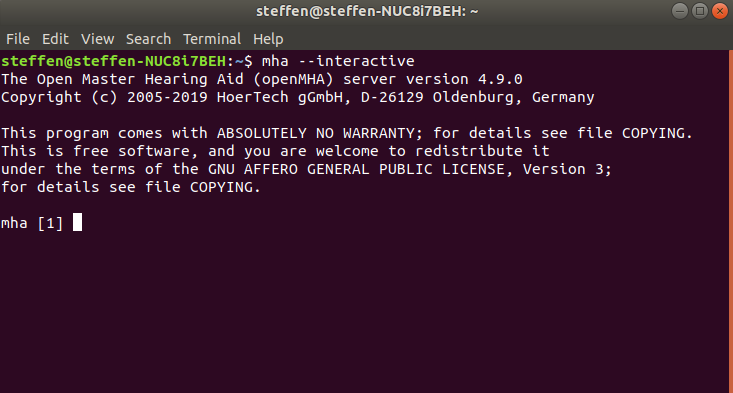
\includegraphics[scale=0.4]{mha_interactive.png}
\caption{- Linux Terminal: Type {{\ttfamily \textbf{mha \texttt{-{}-}interactive}}}}
\end{figure}


\dotfill \\

\large{\textbf{Note}}:
The current directory of the terminal becomes the
current working directory (CWD) of the openMHA process.
openMHA resolves relative file names relative to the CWD.
If in some of the following examples in this guide
openMHA raises an error because it cannot find some file,
check that the file name can be resolved from the CWD.
To fix file lookup problems, either change the CWD in the
terminal before restarting the openMHA, or adapt any file
names to include correct absolute or relative paths.
\\

\textcolor{orange}{\textbf{You have managed to start openMHA. In the next section there will be a step-by-step tutorial on how to use a simple configuration.}}

\vspace{1cm}

In order to terminate the openMHA started in this chapter,
you can type \\
$\rightarrow$ {\ttfamily \textbf{cmd=quit}} \\
followed by \textbf{Enter} into the terminal.



\newpage
\begin{comment}
\section{Use Matlab Function "jack\_playrec" to Communicate with JACK Server}   

One possibility to transfer audio signals to a JACK server is the jack\_playrec. To do this following the steps below:

\begin{enumerate}
\item Start a JACK server (sample rate = 44100)
\item Check if you already followed the instructions from \textbf{section \ref{sec:beforeplayrec}}
    \item \textbf{Start Matlab} 
    \item \textbf{Go to} $\rightarrow$ \textbf{/Users/usr/local/lib YourUserName/usr/local/lib Documents/usr/local/lib jack-playrec/usr/local/lib mfiles}
      using the Matlab/Octave \textbf{"Current Folder"} control
    
      You can now copy the following lines of code into the Matlab/Octave command windows.
      This simple code below shows a minimal example of how to send an audio signal to a JACK client (here system:playback\_1). 


\begin{verbatim}
sampling_rate = 44100; %needs to fit sample rate of JACK server
frequency = 440; %Frequency in Hertz
signal_duration = 1; %Signal duration in seconds

t= 0:1./sampling_rate:signal_duration-1./sampling_rate;
sinus = transpose(sin(2*pi*frequency*t));
jack_playrec(sinus,'output',{'system:playback_1'});
\end{verbatim}  

\end{enumerate}


\newpage
\end{comment}

\section{Step-by-Step Exercise: Gain Application}

\textbf{First Steps}
\label{sec:first_steps}

A simple openMHA use case is the application of a gain to an audio signal.
We will start by applying a gain factor to an audio file named {{\ttfamily \textit{1speaker\_diffNoise\_2ch.wav}}}. The corresponding parameters (e.g. gain factor, input channels, fragment size and sample size) can be set manually, however for this example there is already an openMHA configuration file available at: 
\begin{itemize}\label{list:examples-location}
\item \textcolor{orange}{\textbf{Linux}}: \textit{/usr/share/openmha/examples/00-gain} 
\item \textcolor{orange}{\textbf{Windows}}: \textit{C:\textbackslash Program Files\textbackslash openMHA\textbackslash examples\textbackslash 00-gain}
\item \textcolor{orange}{\textbf{macOS}}: \textit{/usr/local/share/openmha/examples/00-gain} 
\end{itemize}

A shortened version of the gain.cfg file is shown below.
A short description precedes each command
in a line starting with \# which is used for comments.
The actual file on disk contains more verbose comments.
\\

\textbf{gain\_getting\_started.cfg:} \\

\lstinputlisting{../../../examples/00-gain/gain_getting_started.cfg}

\newpage 
In this guide we will use the example files from the openMHA installer.
Since these are installed in a read-only directory, we need to copy
the examples to a writable location before using them. 
Follow these steps:


\begin{enumerate}
    \item \textbf{Close all} running openMHA processes
    
    \item \textbf{Copy} the examples folder from the installation directory
      \\
      (e.g. /usr/share/openmha/examples/)
      (\textcolor{orange}
        {\textbf{see the list on page \pageref{list:examples-location}
            for your specific operating system}})
   
\begin{figure}[H]
\centering
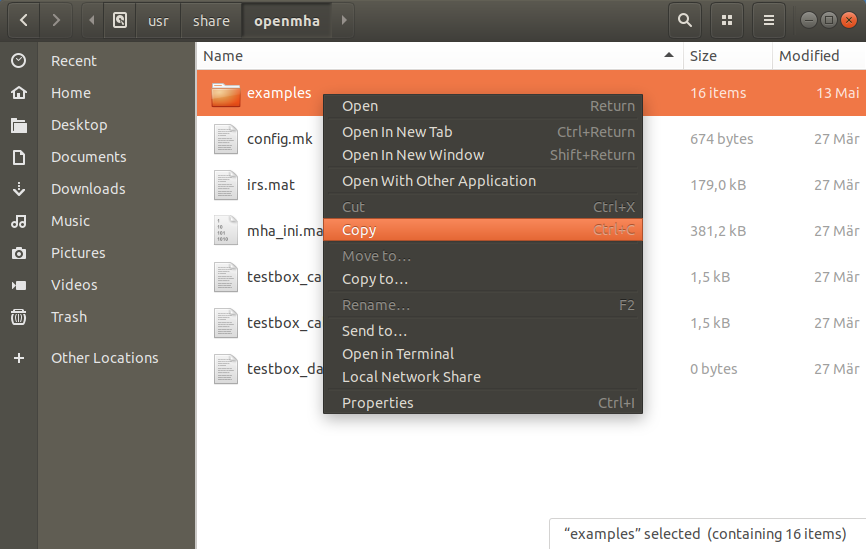
\includegraphics[scale=0.3]{copy_examples.png}
\caption{- Copy the examples folder from the protected directory (e.g. /usr/share/openmha/}
\end{figure}

\item \textbf{Paste} the examples into folder within a writable directory, e.g. your home directory:

\begin{figure}[H]
\centering
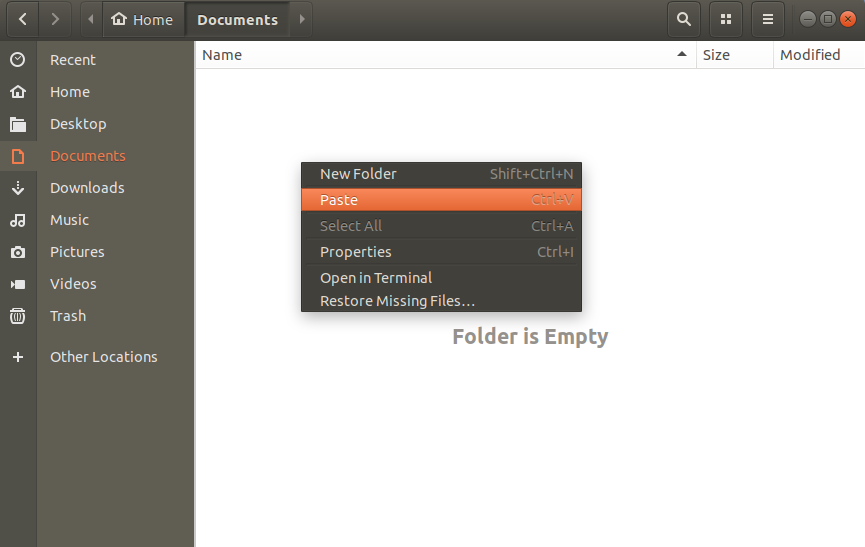
\includegraphics[scale=0.3]{paste_examples.png}
\caption{- Paste examples into folder inside a non-protected directory (e.g. /home/YourUserName/Documents}
\end{figure}
    
    
    \item Open your \textbf{terminal} (see \ref{starting_openmha})
    \item \textbf{Navigate inside the examples folder into the subdirectory of the first example $\rightarrow$ \textbf{00-gain}} \\ (e.g. \textit{/home/YourUserName/Documents/examples/00-gain} )\\ \\
    $\rightarrow$ you can use \textbf{cd ..} to navigate one folder level up \\
    $\rightarrow$ and \textbf{cd foldername} to descend into the subfolder
      \textbf{foldername}\\
    $\rightarrow$ if the \textcolor{orange}{macOS or Linux} terminal does not show the current directory, type \textbf{pwd} \\
    \item Type {{\ttfamily mha \texttt{-{}-}interactive}} and press \textbf{Enter}
\end{enumerate}

\subsection{File to File}

You have started the openMHA in interactive mode and can now type in openMHA commands.
The current working directory of the openMHA should be the copy of the 00-gain example directory in the writable location.
In order to read in the configuration file \textbf{gain.cfg} (which lies directly in \textit{00-gain}), type: \\

%$\rightarrow${\ttfamily ?read:\textbackslash Users\textbackslash YourUserName\textbackslash Documents\textbackslash examples\textbackslash 00-gain\textbackslash gain.cfg}
$\rightarrow${\ttfamily ?read:gain\_getting\_started.cfg}


%with the corresponding file directory of gain.cfg. 
Start the openMHA signal processing by:

$\rightarrow$ {\ttfamily cmd=start}

and then exit openMHA by typing:

$\rightarrow$ {\ttfamily cmd=quit} 
\\

\begin{figure}[H]
\centering
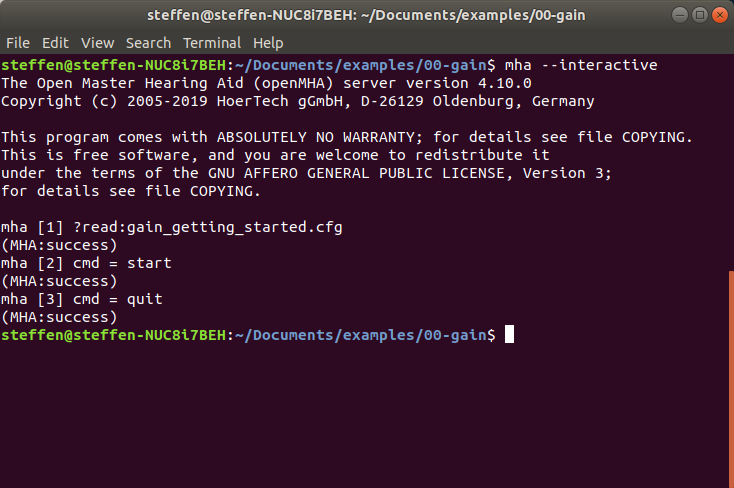
\includegraphics[scale=0.4]{static_gain.png}
\caption{Interactive mode: Applying gain to a static audio signal}
\end{figure}

\textcolor{orange}{\textbf{openMHA has created a second .wav file "1speaker\_diffNoise\_2ch\_OUT.wav" in the current 00-gain folder. (e.g. \textit{/home/YourUserName/Documents/examples/00-gain}). You can listen to it and compare it to "1speaker\_diffNoise\_2ch.wav".}}

\newpage

\subsection{Starting openMHA with JACK Input/Output}

In this section we perform the same signal processing as before, but replace the sound files with the JACK server as audio backend. This means that we can apply a gain to e.g. our microphone input in real time. The configuration file {{\ttfamily \textit{gain\_live.cfg}}} will be used for this. \\

\large{\textbf{Note}}:
This and all following live processing examples configure
the sound card with small buffer sizes. Your combination of
computer, sound card, and operating system may be unable
to process the sound with these settings without dropouts.
If you experience problems, try a faster computer, optimize
the operating system for real-time performance, or use a
different sound card or operating system.
\\

\textbf{gain\_live\_getting\_started.cfg:} \\

\lstinputlisting{../../../examples/00-gain/gain_live_getting_started.cfg}



In order to set up and connect a JACK server you can follow the steps below:

\begin{enumerate}
    \item \textbf{Start Jack Audio Connection Kit} 
    
    \begin{itemize}
\item \textcolor{orange}{\textbf{Linux}}: \\ Type {\ttfamily qjackctl} into your \textbf{terminal}. 
\item \textcolor{orange}{\textbf{Windows}}: \\ Use the \textbf{JACK Control} start menu entry.
\item \textcolor{orange}{\textbf{macOS}}: \\ \textbf{Start} the \textbf{Jack Audio Connection Kit} GUI by starting the \textit{qjackctl} application found in \textit{/Applications/Jack/}.
\end{itemize}

\begin{figure}[H]
\centering
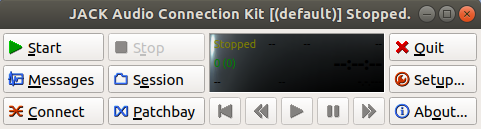
\includegraphics[scale=0.4]{jack_gui.png}
\caption{JACK Audio Connection Kit: GUI}
\end{figure}
      
    \item \textbf{Setup} $\rightarrow$ \textbf{Settings} $\rightarrow$ select proper Driver, Interface, Sample Rate=44100, \\Frames/Period=64 $\rightarrow$ \textbf{OK} 
    
\begin{figure}[H]
\centering
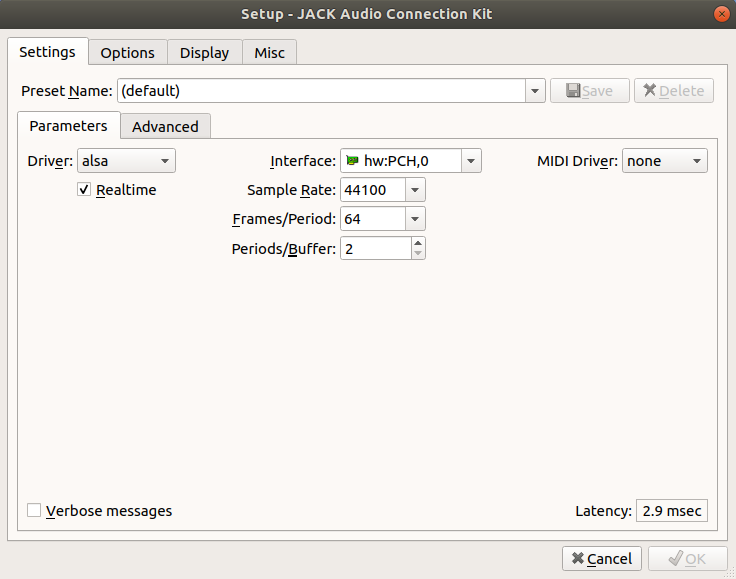
\includegraphics[scale=0.4]{jack_setup.png}
\caption{Jack GUI: Setup}
\end{figure}
    \item Click \textbf{Start} for starting a JACK server $\rightarrow$ Check \textit{Messages} for any errors (sometimes it can be difficult to find proper driver settings, try out different settings) \\
    
\begin{figure}[H]
\centering
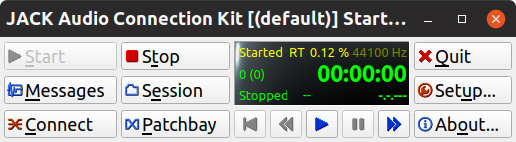
\includegraphics[scale=0.4]{jack_started.png}
\caption{Jack GUI with running server}
\end{figure}

    %\textcolor{red}{\textbf{For macOS Users: If you encounter any problem using JACK you can try \textit{\textbf{JackPilot}}, you can find the download link in section \ref{subsec:required_prog}}}
    


\item In order to test your Jack server, you can go to the \textbf{Connect} section and connect the inputs of your (internal) microphones to the output channels of the jack server (see Figure \ref{fig: jack_connection}).

\begin{figure}[H]
\centering
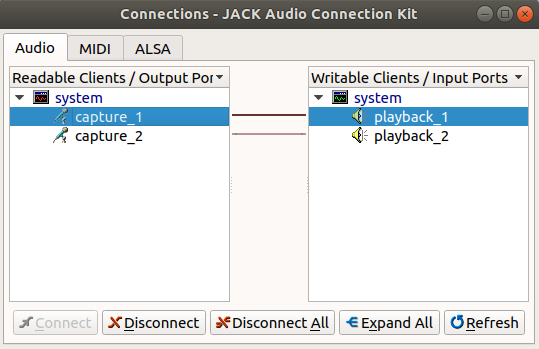
\includegraphics[scale=0.4]{jack_connection.png}
\caption{Jack GUI: Setup}
\label{fig: jack_connection}
\end{figure}


Disconnect these connections again before proceeding.
You can now use the JACK server as audio backend.
To do this, start openMHA in the same directory as before:

\item Open your \textbf{terminal} (see \ref{starting_openmha})
    \item \textbf{Navigate inside the examples folder into the subdirectory of the first example $\rightarrow$ \textbf{00-gain}} \\ 
    \item Type {{\ttfamily mha \texttt{-{}-}interactive}} and press \textbf{Enter}
 
    \item $\rightarrow$ {\ttfamily ?read:gain\_live\_getting\_started.cfg}
    \item $\rightarrow$ {\ttfamily cmd=start}

\mha{} is now applying a gain to your own voice input. In order to close openMHA type:
\item  $\rightarrow$ {\ttfamily cmd=quit}

\end{enumerate}

\textcolor{orange}{\textbf{You have now managed to start some simple
    configurations for a static audio file as well as a live input using Jack.
    In the next session Matlab or Octave will be used as user interface for openMHA.}}

\newpage


\section{Control Frequency Shifter using Octave/Matlab GUI}
\label{sec:freqshifter}


\begin{enumerate}
\item \textbf{End} all running \textbf{mha processes} 
\item \textbf{Open Matlab or Octave} 
\item \textcolor{orange}{\textbf{Linux:}} Set LD\_LIBRARY\_PATH to empty by typing \\ {\ttfamily
  $\rightarrow$ setenv(\textquotesingle
  LD\_LIBRARY\_PATH\textquotesingle,\textquotesingle\textquotesingle)} \\
  into the \textbf{Command Window} \\
\textcolor{orange}{\textbf{MacOS only:}} \\Type: \\{\ttfamily $\rightarrow$ setenv(\textquotesingle PATH\textquotesingle, [getenv(\textquotesingle PATH\textquotesingle) \textquotesingle :/usr/local/bin\textquotesingle]);} \\
into the \textbf{Command Window} \\  
\item Use the Matlab/Octave \textbf{"Current Folder"} control to navigate to:

\begin{itemize}
\item \textcolor{orange}{\textbf{Linux}}: \\
  \textit{/usr/share/openmha/examples/05-frequency-shifting}
\item \textcolor{orange}{\textbf{Windows}}: \\
  \textit{C:\textbackslash Program Files\textbackslash openMHA\textbackslash examples\textbackslash 05-frequency-shifting}
\item \textcolor{orange}{\textbf{macOS}}: \\
  \textit{/usr/local/share/openmha/examples/05-frequency-shifting}
\end{itemize}

\item In order to use the Matlab functions of openMHA type the following using the \textbf{Command Window:} 

\begin{itemize}
\item \textcolor{orange}{\textbf{Linux}}: \\ $\rightarrow$
  {\ttfamily addpath(\textquotesingle{}/usr/lib/openmha/mfiles\textquotesingle{})}
\item \textcolor{orange}{\textbf{Windows}}: \\ $\rightarrow$
  {\ttfamily addpath(\textquotesingle{}C:\textbackslash Program Files\textbackslash openMHA\textbackslash mfiles\textquotesingle{})}
\item \textcolor{orange}{\textbf{macOS}}: \\ $\rightarrow$
  {\ttfamily addpath(\textquotesingle{}/usr/local/lib/openmha/mfiles/\textquotesingle{})}
\end{itemize}


\item In order to start a new openMHA instance type \\
  $\rightarrow$ {\ttfamily openmha = mha\_start;}
\item In order to read in the configuration file type: \\
  $\rightarrow$ {\ttfamily mha\_query(openmha,\textquotesingle{}\textquotesingle{},\textquotesingle{}read:fshift\_live.cfg\textquotesingle{});}
\item \textbf{Start JACK Server} using \textbf{JACK Control}\\
  (Setting: Sample Rate = 44100, Frames/Period = 64)
\item Start the mha process by typing \\ $\rightarrow$
  {\ttfamily mha\_set(openmha, \textquotesingle{}cmd\textquotesingle{},
                      \textquotesingle{}start\textquotesingle{} );}
\item \textbf{JACK Control}: Connect the "capture" and "playback" channels
  of the sound card to the MHA "in" and "out" channels.
  Connect a microphone to the soundcard.
\item Start GUI by typing \\ $\rightarrow$
  {\ttfamily mhagui\_generic(openmha)} into the \textbf{Command Window}
\begin{enumerate}
\item \textbf{mha ->open sub-parser}
\item \textbf{mhachain ->open sub-parser}
\item \textbf{fshift\_hilbert ->open sub-parser}
\item \textbf{df -> open vector<float>control}
\end{enumerate}
\item Change the settings df, fmin and fmax in the GUI and listen to the
  processed microphone sound.
  You can not only move the sliders using the mouse cursor or up- and
  down-arrow keys, but also replace the numbers directly
  by typing new numbers and pressing \textbf{Enter}
  in the text fields of the GUI.
  These settings control a frequency shifter, which band is shifted and how
  much.
\end{enumerate}

\newpage

\section{Control Dynamic Compression using Octave/Matlab GUI}

\begin{enumerate}
\item \textbf{End} all running \textbf{mha processes} (You can type \textbf{killall mha} in the terminal to any running mha processes [Linux/macOS only])
\item \textbf{Open Matlab or Octave}
\item \textcolor{orange}{\textbf{Linux:}} Set LD\_LIBRARY\_PATH to empty by typing \\ {\ttfamily
  $\rightarrow$ setenv(\textquotesingle
  LD\_LIBRARY\_PATH\textquotesingle,\textquotesingle\textquotesingle)} \\
  into the \textbf{Command Window} \\
\textcolor{orange}{\textbf{MacOS only:}} \\Type: \\{\ttfamily $\rightarrow$ setenv(\textquotesingle PATH\textquotesingle, [getenv(\textquotesingle PATH\textquotesingle) \textquotesingle :/usr/local/bin\textquotesingle]);} \\
into the \textbf{Command Window} \\  
\item Use the Matlab/Octave \textbf{"Current Folder"} Section to navigate to:

\begin{itemize}
\item \textcolor{orange}{\textbf{Linux}}: \textit{/usr/share/openmha/examples/01-dynamic-compression} 
\item \textcolor{orange}{\textbf{Windows}}: \textit{C:\textbackslash Program Files\textbackslash openMHA\textbackslash examples\textbackslash 01-dynamic-compression}
\item \textcolor{orange}{\textbf{macOS}}: \textit{/usr/local/share/openmha/examples/01-dynamic-compression} 
\end{itemize}

\item In order to use the Matlab functions of openMHA type the following using the \textbf{Command Window:} 

\begin{itemize}
\item \textcolor{orange}{\textbf{Linux}}: {\ttfamily addpath(\textquotesingle{}/usr/lib/openmha/mfiles\textquotesingle{})}
\item \textcolor{orange}{\textbf{Windows}}: {\ttfamily addpath(\textquotesingle{}C:\textbackslash Program Files\textbackslash openMHA\textbackslash mfiles\textquotesingle{})}
\item \textcolor{orange}{\textbf{macOS}}: {\ttfamily addpath(\textquotesingle{}/usr/local/lib/openmha/mfiles/\textquotesingle{})}
\end{itemize}


\item In order to start openMHA type {\ttfamily openmha = mha\_start;} 
\item Read in configuration into mha by \\ {\ttfamily mha\_query(openmha,\textquotesingle{}\textquotesingle{},\textquotesingle{}read:dynamiccompression\_live.cfg\textquotesingle{});}
\item \textbf{Start JACK Server} using \textbf{JACK Control}\\ (Setting: Sample Rate = 44100, Frames/Period = 64)

\item In order to start the mha process type {\ttfamily mha\_set(openmha,\textquotesingle{}cmd\textquotesingle{},\textquotesingle{}start\textquotesingle{});}


\item The current gaintable {\ttfamily gtdata} and relevant parameters such as {\ttfamily gtmin} and {\ttfamily gtstep} (more information on these can be found under {\url{%
          {http://www.openmha.org/docs/openMHA_plugins.pdf#subsection.2.1}}}
\large) can be read out by: \\

{\ttfamily gaintable = mha\_get(openmha,\textquotesingle{}mha.overlapadd.mhachain.dc.gtdata\textquotesingle{});}\\
{\ttfamily gtmin = mha\_get(openmha,\textquotesingle{}mha.overlapadd.mhachain.dc.gtmin\textquotesingle{});}\\
{\ttfamily gtstep = mha\_get(openmha,\textquotesingle{}mha.overlapadd.mhachain.dc.gtstep\textquotesingle{});}



The variables {\ttfamily gtmin} (minimum input level) and {\ttfamily gtstep} (input level increment) expect vectors, but we have assigned scalar values to {\ttfamily gtmin} and {\ttfamily gtstep} previously. Scalar values will be interpreted as vectors of length 1 by the MHA when assigned to vector variables. The dc plugin allows vectors of length 1 for variables {\ttfamily gtmin} and {\ttfamily gtstep}, in this case the same value applies to every channel/band. It is also possible to have different {\ttfamily gtmin}/{\ttfamily gtstep} values for each channel/band by assigning a vector of values to these variables where the number of elements in the vector is equal to the number of channels/bands.

\item You can design your own gaintable in Matlab, e.g. noise gate, compressive region, output limit \\
  {\ttfamily gaintable = repmat([-50,30:-2:0,-4:-4:-32],18,1);} \\
  with \\
  {\ttfamily gtmin = zeros(1,size(gaintable,1));} \\
  and \\
  {\ttfamily gtstep = 4*ones(1,size(gaintable,1));} 
  

This would result in an input/output characteristic which is the same for every channel/band.

\item Plot the I/O characteristics \\
{\ttfamily level\_in = ((1:size(gaintable,2))-1) .* gtstep\textquotesingle{}+gtmin\textquotesingle{};}\\
{\ttfamily level\_out = level\_in + gaintable;}

\item In order to apply the gaintable type \\
{\ttfamily mha\_set(openmha,\textquotesingle{}mha.overlapadd.mhachain.dc.gtdata\textquotesingle{},gaintable);}
\item In order to plot input and output level in Matlab, type \\ {\ttfamily figure, plot(level\_in\textquotesingle{},level\_out\textquotesingle{})}

\textcolor{orange}{Note: You can also use the mfile tool \textbf{dc\_plot\_io.m}}. For this type: 

{\ttfamily figure, dc\_plot\_io(gtmin, gtstep,gaintable, level\_in);}


\item You can design more gaintables in Matlab, e.g. by using 
  {\ttfamily gaintable\_new = [...]}
  \begin{itemize}
  \item e.g. Squash all input levels to the same output level, infinite compression:
    \\ \texttt{gaintable\_new = 65.*ones(18,1) - level\_in;}
  \item e.g. compress high frequency band only: ...
  \end{itemize}
\item In order to apply the new gaintable type \\
{\ttfamily mha\_set(openmha,\textquotesingle{}mha.overlapadd.mhachain.dc.gtdata\textquotesingle{},gaintable\_new);}
\item The fitting GUI can be started by typing {\ttfamily mhacontrol(openmha)}
\item You can stop openMHA using {\ttfamily mha\_set(openmha,\textquotesingle{}cmd\textquotesingle{},\textquotesingle{}quit\textquotesingle{})}



\end{enumerate}
\newpage
\section{Using AC Variables}
\label{sec:ac_variables}

The objective of this section is to learn about dealing with AC-Variables in combination with Matlab. \\ \\

\textbf{What are AC Variables?} \\

Sometimes plugin algorithms need to share more information than just the current audio signal. \mha{} supports this by providing a mechanism to share any type of additional data between plugins in the form of \textcolor{orange}{\textbf{algorithm communication variables}} or \textcolor{orange}{\textbf{AC variables}}. Further information on the purpose of AC Variables can be found in the \textit{Application Manual} section~2.2. \\

\dotfill \\

The coherence between two live microphone signals is investigated. A JACK server is used to connect both microphone signals to openMHA.  

\begin{enumerate}

\item \textbf{Start JACK Server} using \textbf{JACK Control}\\
  (Setting: Sample Rate = 44100, Frames/Period = 64) \\
  \textcolor{red}{\textbf{Note: You need to have \underline{two microphone inputs} available for this task}}

\item Start Matlab/Octave and the \textbf{"Current Folder"} control to navigate to: 

\begin{itemize}
\item \textcolor{orange}{\textbf{Linux}}: \textit{/usr/share/openmha/examples/15-ac-variables} 
\item \textcolor{orange}{\textbf{Windows}}: \textit{C:\textbackslash Program Files\textbackslash openMHA\textbackslash examples\textbackslash 15-ac-variables}
\item \textcolor{orange}{\textbf{macOS}}: \textit{/usr/local/share/openmha/examples/15-ac-variables} 
\end{itemize}

\item Open the Matlab script \textbf{\textit{acmatlab.m}} \\

The most important lines of \textbf{acmatlab.m} are shown below:

\begin{Verbatim}[numbers=left,commandchars=\\\{\}]
%Start openMHA process
\textcolor{orange}{\textbf{openmha = mha_start;}}
% Read configuration file
\textcolor{orange}{\textbf{mha_query(openmha,'','read:coherence_live.cfg');}}
% Start configuration file
\textcolor{orange}{\textbf{mha_set(openmha,'cmd','start')}}

%% Label center frequencies and set gain factor of ac_proc

% Label center frequencies
\textcolor{orange}{\textbf{freqs=mha_get(openmha,'mha.overlapadd.mhachain.coherence.cf'); 
}} 
% Set gain factor in dB - default value was choosen to be 6
\textcolor{orange}{\textbf{mha_set(openmha,'mha.overlapadd.mhachain.coh_gain.gain.gains',6);}}
\end{Verbatim} 



%mha_get(openmha,'mha.overlapadd.mhachain.acmon')
\newpage

\textbf{Explanation}

The configuration used is called \textit{coherence\_live.cfg}. It uses the plugin \textbf{mhachain} in order to connect three plugins: \\
1. coherence \\
2. ac\_proc:coh\_gain \\
3. acmon in series. \\
Within the configuration file this is denoted by: \\

{\ttfamily mha.overlapadd.mhachain.algos = [coherence ac\_proc:coh\_gain acmon]} \\



 The purpose of each plugin is the following: \\

\textbf{coherence:} This plugin measures the coherence between the two microphone input signals. \\ \\
\textbf{ac\_proc:coh\_gain:} The real name of the plugin is \textit{ac\_proc}, however in this case the alias \textit{coh\_gain} is used. This plugin interprets the AC variable data stream received from \textit{coherence} as an audio signal. The plugin itself can load another plugin. In this case the gain plugin is loaded. The gain factor was choosen to be 6 dB. This means that the AC variable output "signal" is amplified by 6 dB. (line 12) Outside the plugin ac\_proc the signal is provided as AC variable stream.\\ \\
\textbf{acmon:} This plugin is used to convert incoming AC variable data streams into monitor variables. In this case the output of \textit{coherence} as well as \textit{ac\_proc:coh\_gain} is used.

\begin{figure}[H]
\centering
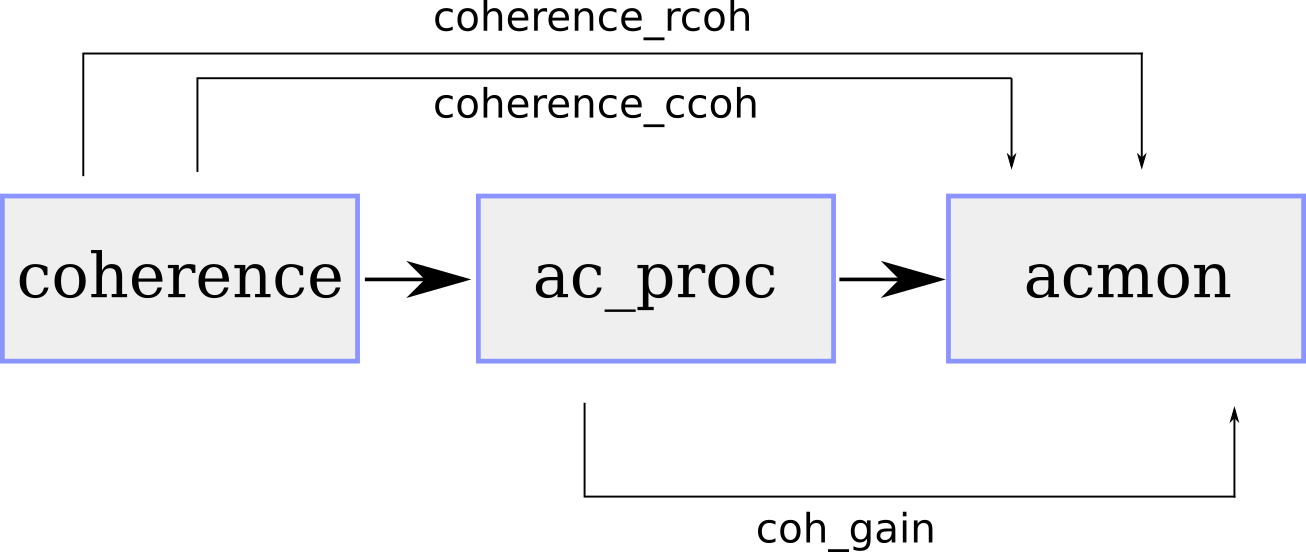
\includegraphics[scale=0.7]{coherence_chain.png}
\caption{Schematics of AC variable data stream between plugins: coherence, ac\_proc, acmon}
\end{figure}


\newpage
\item Start the Matlab script \textbf{acmatlab.m}

\begin{figure}[H]
\centering
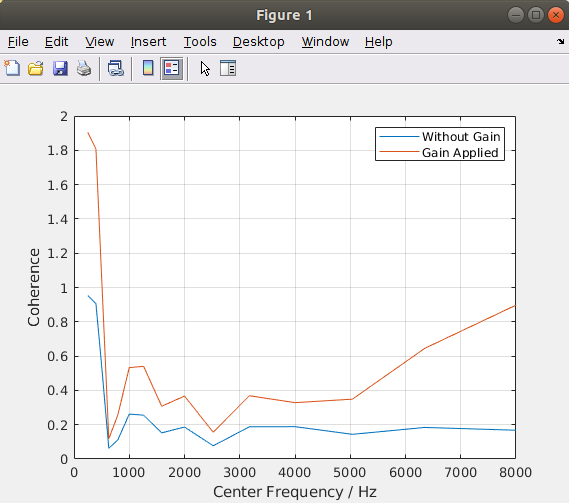
\includegraphics[scale=0.5]{ac_variables_coherence.png}
\caption{Matlab: Coherence plotted as a function of frequency}
\end{figure}

The purpose of this example is to show that the plugin ac\_proc can be used to apply common signal processing operations such as a gain to an originally non-audio signal such as an AC variable data stream.
\end{enumerate}







\newpage

\section{Writing your own Configuration Script}
\label{sec:own_config_script}

This section will offer a guide on how to write your own openMHA script. For doing so some basic parameters need to be set. In this example we want to write an example script for using the \textit {sine} plugin. \\



First it is necessary to fix the following parameters:

\begin{enumerate}
\item \textbf{Number of input channels} ({\ttfamily nchannels\_in})
\item \textbf{Fragment size} ({\ttfamily fragsize})
\item \textbf{Sampling rate in Hz} ({\ttfamily srate}) 

For an input file with two channels and a sampling rate of 44.1 kHz. This could for example look like: \\

\lstinputlisting[firstline=1,lastline=6,numbers=none]{./example_script.cfg}



\item \textbf{Plugin(s):} Next we need to tell the MHA which plugin(s) to load with the {\ttfamily mhalib} variable. As mentioned in the beginning of the section the sine plugin will be used as an example: \\

\lstinputlisting[firstline=7,lastline=8,numbers=none]{./example_script.cfg}

\item \textbf{Configuration variables:} Each plugin has \textit{configuration variables} which can be adjusted accordingly. For each plugin the configuration variables are listed in the \textit{plugin manual} 
\\(\footnotesize{\url{%
          {http://www.openmha.org/docs/openMHA_plugins.pdf#subsection.16.3}}}
\normalsize for sine plugin). These variables can be adjusted according to your requirements, such as the frequency of the sine wave ({\ttfamily f}), the RMS level ({\ttfamily lev}) or if the input signal should be added to the sine wave or replaced completely ({\ttfamily mode}). An extract from the \textit{plugin manual} is shown below in Figure \ref{fig:config_variables_sine}. 

\begin{figure}[H]
\centering
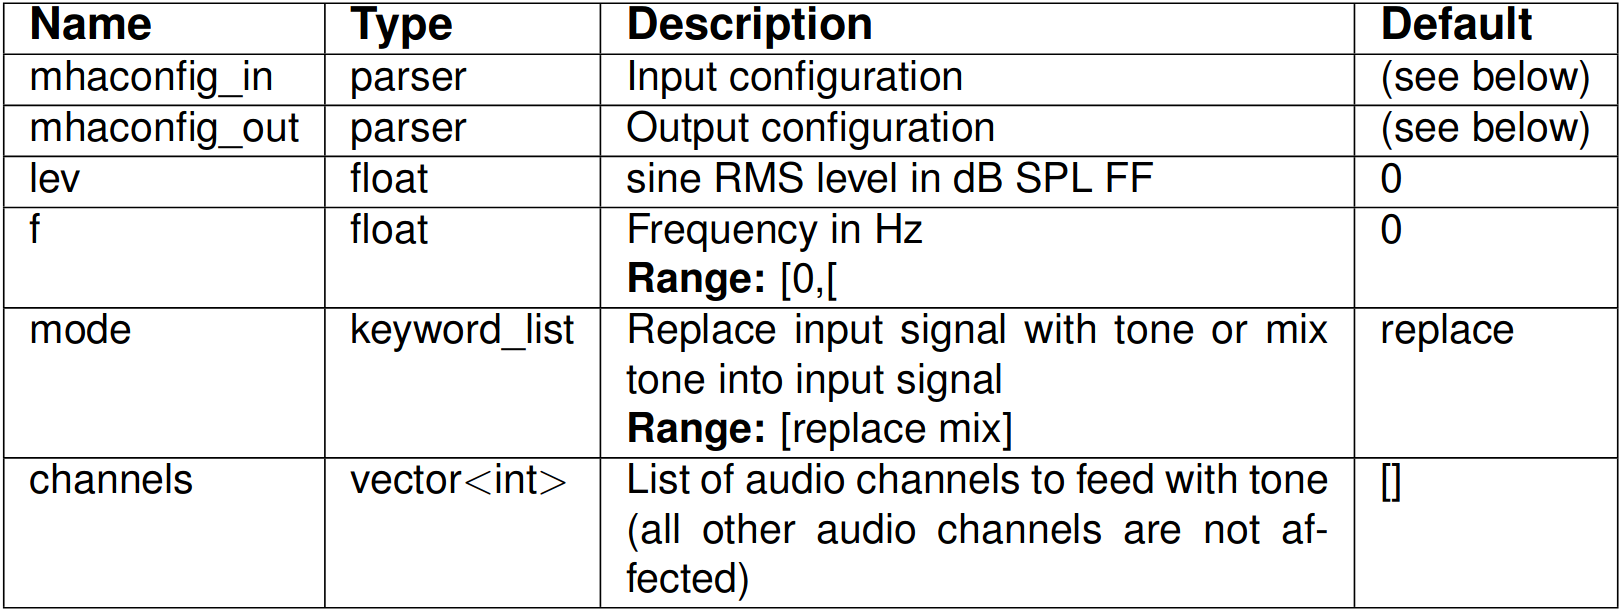
\includegraphics[scale=0.22]{config_variables_sine.png}
\caption{Extract from \textit{Plugin Manual}: Configuration variables of the
         \texttt{sine} plugin}
\label{fig:config_variables_sine}
\end{figure}

Although the plugin is used by {\ttfamily mhalib = sine}, the variables of the plugin are changed by setting {\ttfamily mha.<variable\_name>~=~value}. This could for example look like:

\lstinputlisting[firstline=9,lastline=17,numbers=none]{./example_script.cfg}

Here the frequency was adjusted to 440 Hz and the RMS level of the sine tone was changed to 100 dB. The operating mode was to set to {\ttfamily mix}, such that the input is mixed with the sine signal (instead of being replaced). The variable {\ttfamily channels} was adjusted to [0]. This means that the sine plugin is only operating on the first channel. In order to operate on both channels {\ttfamily mha.channels~=~[0 1]} can be used.  
           

\item \textbf{Audio Back-End:} openMHA supports different audio back-ends, such as sound drivers, JACK audio servers, sound files or networks. This can be adjusted by choosing the so called IO plugin library ({\ttfamily iolib}). : \\ \\For static audio files: 
{e.g. \ttfamily iolib = MHAIOFile}\\
For live JACK signals: 
{\ttfamily iolib = MHAIOJack}\\
In this case we want to work with a static audio file such that we need to choose: \\

\lstinputlisting[firstline=19,lastline=20,numbers=none]{./example_script.cfg}

\item \textbf{Input} ({\ttfamily io.in}) \\ \\For static audio files: 
{\ttfamily io.in = name\_of\_file.wav}\\
For live JACK signals: 
{\ttfamily io.con\_in = [system:capture\_1 system:capture\_2]} \\
(for two input channels)

\lstinputlisting[firstline=21,lastline=24,numbers=none]{./example_script.cfg}

\textcolor{red}{\textbf{Note: In this case the input file needs to be in the same directory as the .cfg file itself. If this is not the case the absolute or relative (to the .cfg file) path can be used, e.g.}}

\begin{itemize}
\item {\ttfamily ./../Folder/1speaker\_diffNoise\_2ch.wav} (\textit{relative path})
\item {\ttfamily /home/UserName/Folder/1speaker\_diffNoise\_2ch.wav} (\textit{absolute path})
\end{itemize} 

\newpage

\item \textbf{Output} ({\ttfamily io.out}) \\ \\For static audio files: 
{e.g. \ttfamily io.out = name\_of\_file\_out.wav}\\
For live JACK signals: 
{\ttfamily io.con\_out = [system:playback\_1 system:playback\_2]}\\
(for two output channels)

\lstinputlisting[firstline=25,lastline=26,numbers=none]{./example_script.cfg}

\end{enumerate}

\textit{How to run your script:}

\begin{enumerate}
\item Start openMHA in the \textbf{same directory} as your .cfg file
\item $\rightarrow${\ttfamily ?read:your\_script.cfg}
\item Start the openMHA signal processing by:

$\rightarrow$ {\ttfamily cmd=start}

\item In order to exit openMHA type:

$\rightarrow$ {\ttfamily cmd=quit} 
\\
\end{enumerate}

\end{document}

%%% Local Variables: 
%%% mode: latex
%%% TeX-master: "openMHA_application_manual"
%%% indent-tabs-mode: nil
%%% coding: utf-8-unix
%%% End:
